\documentclass[12pt]{article}
\usepackage{fullpage}
\usepackage{enumitem}
\usepackage{graphicx}
\usepackage{listings}
\lstset{language=c, numbers=left}

\newcommand{\SSBC}{SSBC-1}
\begin{document}
\title{Simulated Single Board Computer\footnote{The SSBC library, starter code, and documentation \copyright 2020, Christopher A. Bohn}}
\author{\SSBC}
\date{}
\maketitle

The \SSBC\ is the latest product from Exciting Emulations\footnote{Exciting
Emulations is a wholly-figmentary subsidiary of Babbage's Analytic Engines, a
Limited-Reality Corporation.} and is guaranteed to bring you minutes of fun.
The finest piece of simulated hardware, the \SSBC\ is second only to actually
placing your hands on a real, physical single board computer.

In using the \SSBC, you will have the opportunity to use inputs such as
simulated toggle switches and a simulated numeric keypad, and you will have the
opportunity to create output via simulated seven-segment displays.

\section{Overview}

\begin{figure}
    \centering
    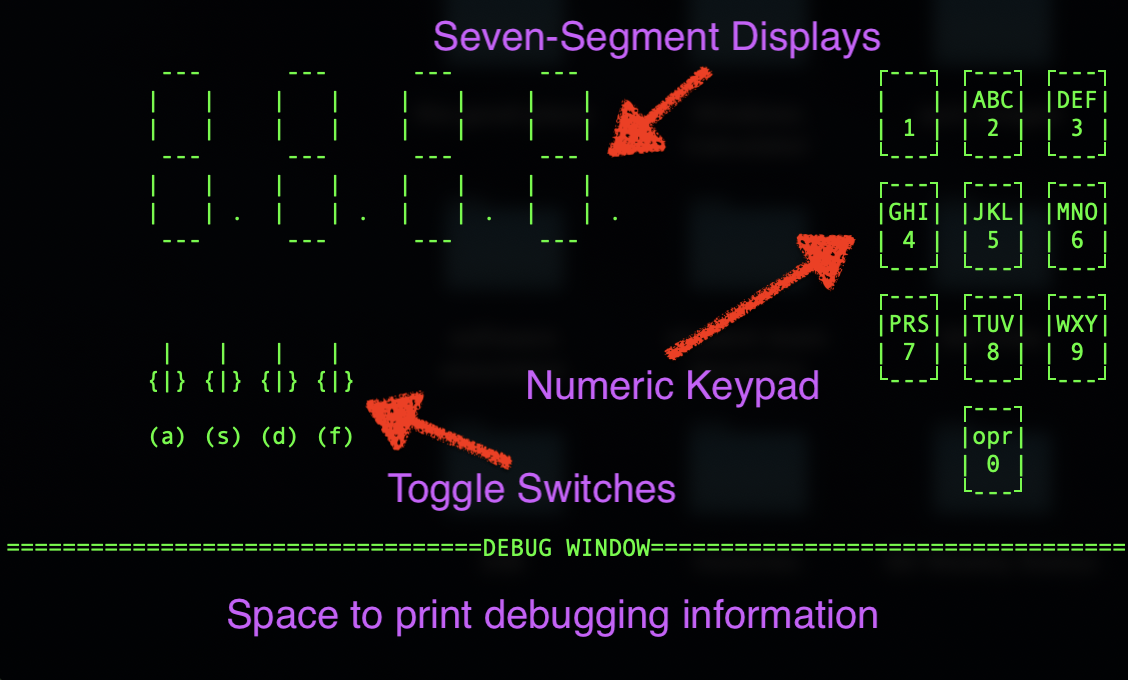
\includegraphics[width=15cm]{overview}
    \caption{Overview of \SSBC.\label{fig:overview}}
\end{figure}

As shown in Figure~\ref{fig:overview}, the \SSBC\ includes a numeric keypad and
four toggle switches for input, and four seven-segment displays for output.
Unlike a real single board computer, you will not have your \SSBC\ attached to a
separate general-purpose computer for side-loading and debugging, and so the
\SSBC\ also includes a small space for you to print information to help you
debug your programs. \textbf{\textit{Note:} your terminal window must be at
least $24 \times 80$ for \SSBC.} A larger terminal window will also work, but
smaller terminal window will give you an unsatisfactory experience.

\begin{figure}
    \centering
    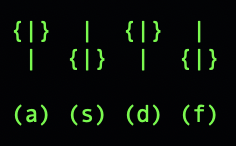
\includegraphics[width=5cm]{toggles}
    \caption{Toggle switches.\label{fig:toggles}}
\end{figure}

The toggle switches (Figure~\ref{fig:toggles}) can be placed in one of two
positions, and a toggle switch will hold its position until it is placed in the
other position. You can toggle a switch by pressing the letter on your keyboard
that corresponds to the switch. For example, the leftmost switch can be placed
in the ``up'' position by pressing \texttt{a}, and then it can be returned to
the ``down'' position by pressing \texttt{a} again.

\begin{figure}
    \centering
    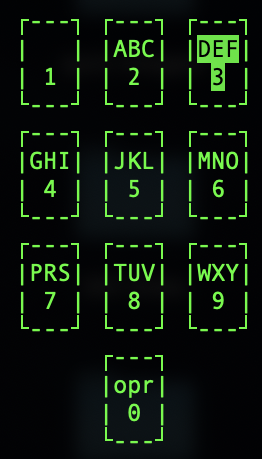
\includegraphics[width=6cm]{keypad}
    \caption{Numeric keypad.\label{fig:keypad}}
\end{figure}

The numeric keypad (Figure~\ref{fig:keypad}) consists of ten momentary buttons,
labeled 0-9. You can depress a number button by pressing the number on your
keyboard that corresponds to the number button. For example, by pressing
\texttt{3}, the upper-left number button will briefly illuminate, and the value
$3$ will be placed in the input register for the numeric keypad. As described
in Section~\ref{sec:keypad}, while depressing the button is momentary, the
value will persist in the input register even after the number button is
released.

\begin{figure}
    \centering
    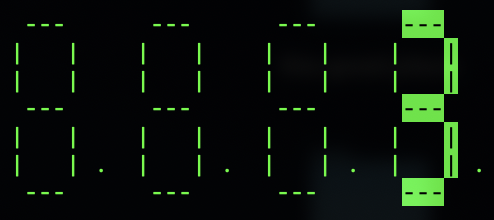
\includegraphics[width=10cm]{7segment}
    \caption{Seven-segment displays.\label{fig:7segment}}
\end{figure}

The seven-segment displays (Figure~\ref{fig:7segment}) consists of seven
segments that can be illuminated or not to create characters, such as the
number $3$, as well as a ``dot'' that can be used for decimal points. The seven-
segment displays will always illuminate their segments in accordance with the
contents of the display register.

\subsection{Other Controls}

In addition to the controls described above, the \SSBC\ will also respond to
these actions on your keyboard:

\begin{figure}
    \centering
    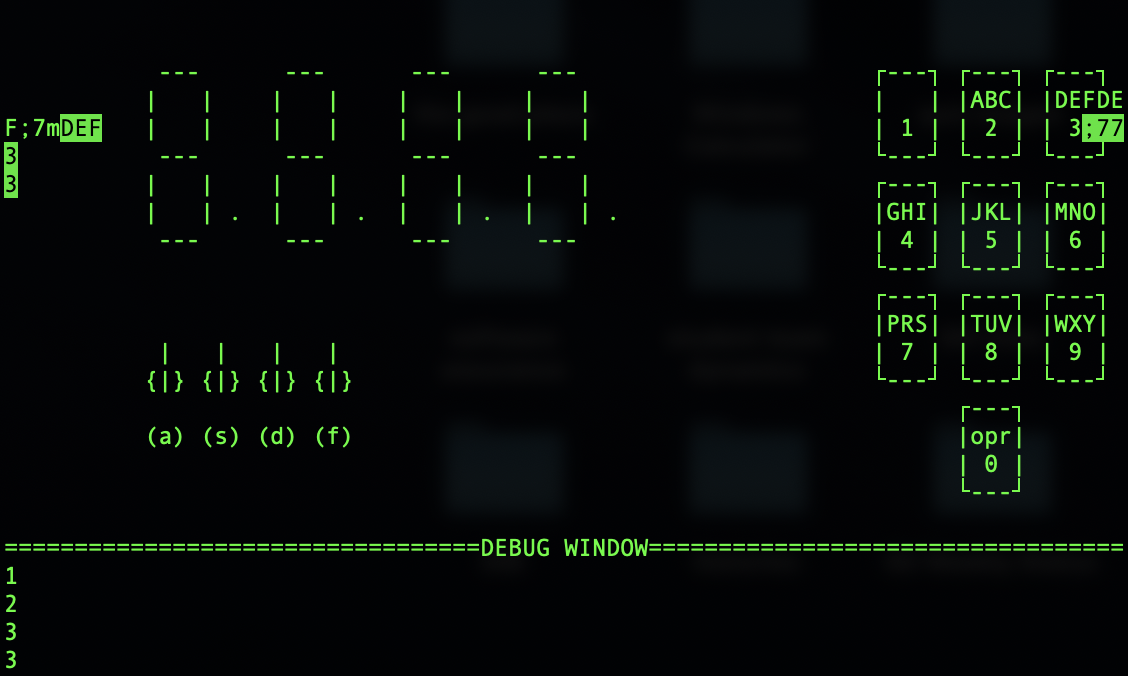
\includegraphics[width=15cm]{garbled}
    \caption{Garbled \SSBC\  screen.\label{fig:garbled}}
\end{figure}

\begin{itemize}
    \item \SSBC\ is an imperfect simulation of a single board computer. If your
        screen becomes garbled (Figure~\ref{fig:garbled}) then you can press
        the \texttt{space} bar to refresh the screen. In extreme cases, you may
        need to press the \texttt{space} bar multiple times. (Under normal
        usage, your screen should not become garbled.)
    \item If you wish to terminate the \SSBC, then press \texttt{Control-C}.
    \item Another way to terminate the \SSBC\ is to type \texttt{quit} with no
        more than 500ms between key presses.
    \item Any other keyboard presses will result in an audio and visual alert
        from \SSBC\ but will otherwise be ignored.
\end{itemize}

\newpage \section{Demonstration Program}

The \texttt{ssbc.h} header file defines seven functions:

\begin{description}
    \item [void ssbc\_launch()] This function should be the first line of your
        program's \texttt{main} function. It will initialize \SSBC\ and generate
        the \SSBC\ screen.
    \item [void ssbc\_terminate()] In addition to the means to terminate \SSBC
        from the keyboard, described earlier, you can also let \SSBC\ terminate
        by having your program end its perpetual loop. If you do this, your
        program should call \texttt{ssbc\_terminate} to restore your terminal
        window's settings.
    \item [pthread\_mutex\_t *ssbc\_get\_mutex()] This function returns a
        mutual exclusion token to manage race conditions in the \SSBC's input/
        output registers.
    \item [int ssbc\_print(const char *fmt, ...)] This function is used to
        print text in the debug window. The specification for the arguments is
        identical to that of \texttt{printf}. \textit{Do not use
        \texttt{printf} for printing while using the \SSBC!} The
        \texttt{ssbc\_print} function returns the number of characters printed
        (which may exceed the available space in the debug window.)
    \item [void *ssbc\_get\_keypad\_address()] This function returns the
        address of the numeric keypad's register.
    \item [void *ssbc\_get\_toggle\_address()] This function returns the
        address of the toggle switches' register.
    \item [void *ssbc\_get\_7\_segment\_address()] This function returns the
        address of the seven-segment displays' register.
\end{description}

The \texttt{demo.c} program demonstrates the use of these functions. When a
toggle switch is moved to the ``on'' position, one of the seven-segment
displays illuminates the letter used to toggle the switch. When a number key is
pressed, the number is printed in the debug menu.

\lstinputlisting{../distribution/demo.c}

Line 5 imports `ssbc.h`; you shouldn't need to import any other headers.

Lines 7-10 declare global variables to hold values obtained from some of the
function calls described earlier. In this example, we could have had these
variables local to \texttt{main}, but some programs will be easier to write if
these variables are global. Notice that we can use pointers to any size of
integer to hold the addresses of \SSBC's input/output registers.

The \texttt{running} variable on line 11 is used as a loop variable on line 22.

Line 14 launches the \SSBC. Line 15 contains the bit vectors that will be used
to display letters on the seven-segment displays. See
Section~\ref{sec:7segment} for a discussion of the bit vectors.

Lines 16-19 populate the variables in lines 7-10. Because this program does not
use the first 16 bits of the numeric keypad's register, line 20 uses pointer
arithmetic to point to the second 16 bits.

Line 21 is a variable to keep track of the last number pressed. Recall that
after a number is pressed, its corresponding value persists in the register.
This means that without further information our program cannot determine
whether the value in the register is a stale value or the result of a new
keypress. In Sections~\ref{sec:keypad} and \ref{sec:numberInterrupt} we will
discuss how to detect that a key has been pressed. For now, \texttt{demo.c}
will ignore a value if it is the same value that was previously read from the
register.

Lines 22-50 are the main loop. A common idiom is to write an infinite loop
using \texttt{while(1)} or \texttt{for(;;)}. Here the loop is conditioned on
the \texttt{running} variable from line 11. This will allow us to write code
that will end the loop due to user input.

Lines 23 \& 26 (along with other lines later in the loop) lock and unlock the
mutual exclusion token. As discussed in Section~\ref{sec:registers}, the \SSBC\
is an imperfect simulation that will require you to use the mutual exclusion
token to guarantee that reading and writing registers is
atomic.\footnote{Students: why do you think this is necessary for a simulated
SBC and not for a real, physical SBC?}

Lines 24 \& 25 read from the input registers, and the loop on lines 27-40
updates the bit vector in the seven-segment displays' register based on the bit
vector read from the toggle switches' register.

If a new number button has been pressed, then line 43 prints the number to the
debug window. Note that this print statement also requires locking and
unlocking the mutual exclusion token.

If that number happened to be $0$ then line 48 sets the \texttt{running}
variable to 0, which will terminate the loop. Once the loop has terminated, the
call to \texttt{ssbc\_terminate} on line 51 restores the terminal window's
original settings.

\newpage \section{Input/Output Register Descriptions} \label{sec:registers}

This section describes the registers of the memory-mapped simulated inputs and
outputs.

\SSBC\ is an imperfect simulation. Unlike physical hardware, the simulated
input hardware is not guaranteed to atomically update the input registers, and
the simulated output hardware is not guaranteed to reflect instantaneous
changes to the output registers. Interleavings with the program may result in
inconsistent updates to and reads from the input/output registers. Moreover,
interleavings with the program may result in the terminal window being
improperly refreshed, such as is shown in Figure~\ref{fig:garbled}. Obtaining
a mutual exclusion lock before accessing a simulated I/O register and releasing
the lock when finished with reading from or writing to the register will result
in atomic reads \& writes. Because the \texttt{ssbc\_print} function also
updates the display, be sure to obtain the lock before printing and release the
lock when finished. \textbf{\textit{Note: }failure to release the lock will
render your program and the \SSBC\ non-responsive.}

In the diagrams that follow, the values on the left indicate each row's address
offset (in bytes) from the register's base address. The values along the top
indicate the bit positions for the fields within the bit vectors.

\subsection{Output Register}

\subsubsection{Seven Segment Displays Register} \label{sec:7segment}

The seven-segment displays (Figure~\ref{fig:7segment}) are numbrered, from
right-to-left $0..3$. Each has a field within the seven-segment displays'
register that is used to illuminate particular segments.

\begin{center}
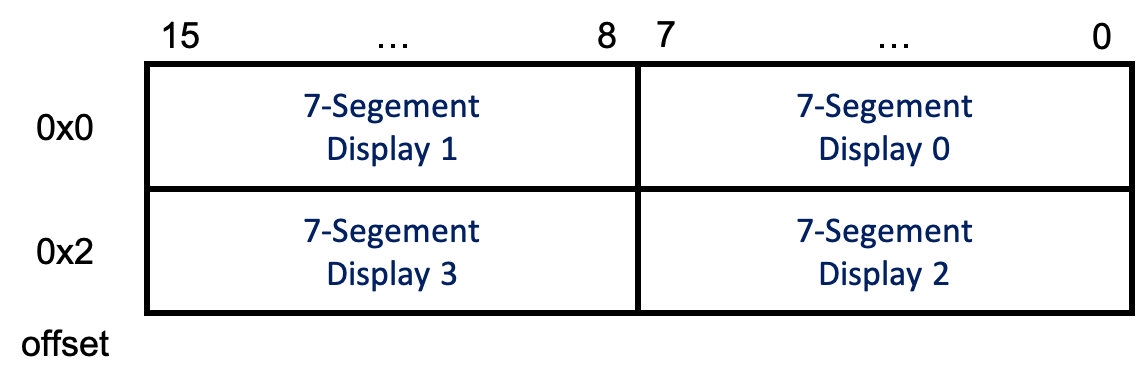
\includegraphics[width=10cm]{7segment-register}
\end{center}

\begin{figure}
    \centering
    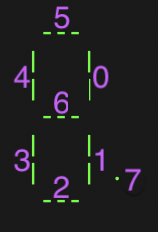
\includegraphics[width=5cm]{7segment-bits}
    \caption{Bits to illuminate each segment for a seven-segment display.\label{fig:7segment-bits}}
\end{figure}

Within each field, the bits that corrsespond to each segment and the dot are
shown in Figure~\ref{fig:7segment-bits}.

\subsection{Input Registers}

\subsubsection{Toggle Switches Register} \label{sec:toggles}

The toggle switches (Figure~\ref{fig:toggles}) are numbered, from
right-to-left, $0..3$. Each has a corresponding bit in the toggle switches'
register that indicates its on/off orientation.

\begin{center}
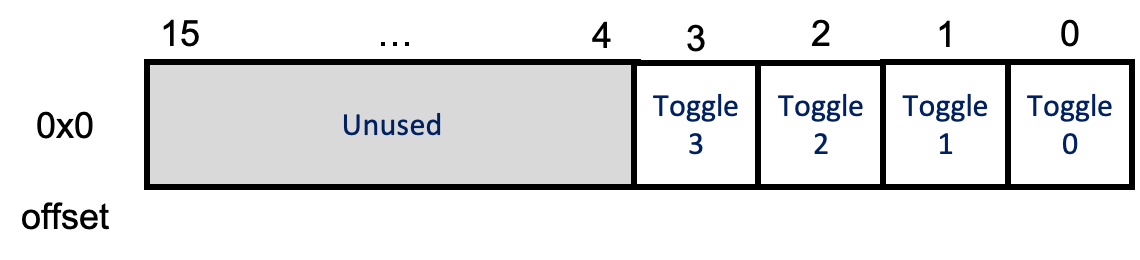
\includegraphics[width=10cm]{toggle-register}
\end{center}

\subsubsection{Numeric Keypad Register} \label{sec:keypad}

When a number button on the numeric keypad is pressed, the binary
representation of that number is placed in the \texttt{BCD value} field of the
numeric keypad register. After the \SSBC\ has been initialized and before any
number buttons have been pressed, the \texttt{BCD value} field will hold a bit
vector that does not correspond to a decimal value. After a number button has
been pressed, the \texttt{BCD value} field will hold the bit vector
corresponding to the last button pressed.

When a number button is pressed, the \texttt{dirty bit} is set to 1. If your
program sets the \texttt{dirty bit} to 0 when the \texttt{BCD value} is read,
then the program can poll the \texttt{dirty bit} to determine whether there has
been a fresh key press.

\begin{center}
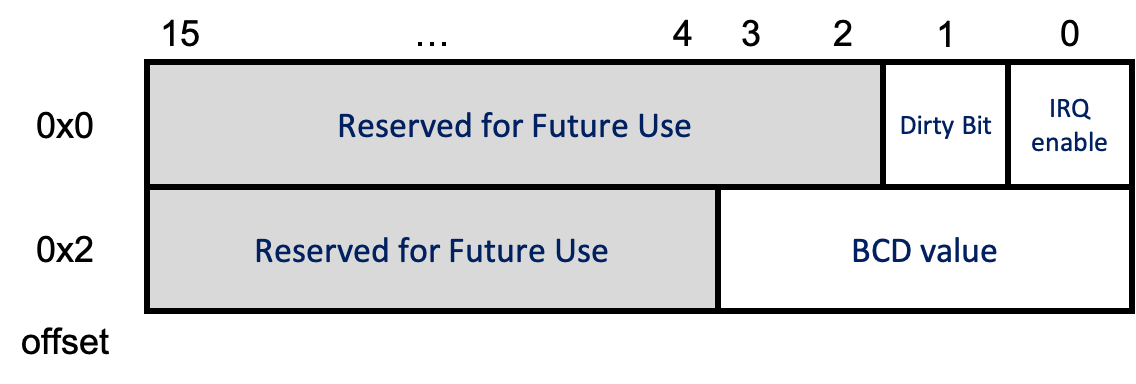
\includegraphics[width=10cm]{keypad-register}
\end{center}

\newpage \section{Simulated Interrupts} \label{sec:interrupts}

The \SSBC\ uses OS signals to simulate hardware interrupts. If you define a
signal handler that returns void and optionally takes an \texttt{int} argument,
and register that signal handler with \texttt{sigset(\textit{signal},
\textit{signal\_handler})} then the signal handler will be called whenever that
signal has been issued.

Register signals only after calling \texttt{ssbc\_launch}, as the \SSBC's
initialization code sets the simulated interrupts to be ignored by default.

\subsection{Numeric Keypad Interrupt} \label{sec:numberInterrupt}

If the numeric keypad register's \texttt{IRQ enable} bit is set, then the
\SSBC\ will issue the \texttt{SIGUSR1} signal whenever a number key has been
pressed. A signal handler registered for \texttt{SIGUSR1} will be called
whenever a number key is pressed, if the \texttt{IRQ enable} bit is set.

\end{document}
